\documentclass[10pt]{article}
\usepackage{geometry}
\usepackage{multirow}
\usepackage{graphicx}
\usepackage{array}
\usepackage{amssymb}
\usepackage{amsmath}
\usepackage{enumitem}
\usepackage{listings}
\usepackage{float}
\usepackage{hyperref}
\usepackage[spanish]{babel}

\title{Tarea 6}
\author{Nicolas Aguilera García - 2127303}
\date{\today}
\geometry{letterpaper, top=2.5cm, bottom=2.5cm, left=3cm, right=3cm}    
\graphicspath{ {./images/} }
\setlength{\parindent}{0cm}
\setlength{\parskip}{0.2em}


\begin{document}
    \maketitle

    \section{Oscilador armónico: el método de Euler y RK2.}
    Para el desarrollo del punto se definieron diferentes funciones, principalmente una para cada una de las ecuaciones diferenciales que representan el oscilador armónico, junto con una función correspondiente al método de Euler y otra para el método de Runge-Kutta.
    
    \begin{verbatim}
// Ecuaciones que representan el movimiento oscilatorio
double dvdt(double t, double x)
{
    return -((k * x) / m);
}

double dxdt(double t, double v)
{
    return v;
}

// Metodo De Euler
double method_euler(double f0, double f, double t, double dt, function<double(double, double)> dfdt)
{
    return f0 + dfdt(t, f) * dt;
}

// Metodo RK-2
double method_runge(double f0, double f, double t, double dt, function<double(double, double)> dfdt)
{
    double k1, k2, ft_1;

    k1 = dfdt(t, f);
    k2 = dfdt(t, f + dt * k1);

    return f0 + (dt / 2) * (k1 + k2);
}
    \end{verbatim}
    
    Utilizando estas funciones y unas condiciones iniciales dadas, 
    
    \begin{itemize}
        \item $x0 = 5$
        \item $v0 = 0$
        \item $m = 1$
        \item $k = 5$
    \end{itemize} 
    
    se construyo la gráfica de trayectorias en donde se presenta el cambio de velocidad y posición en función del tiempo junto con una gráfica que representa el espacio de fases.
    
    \begin{figure}[H]
        \centering
        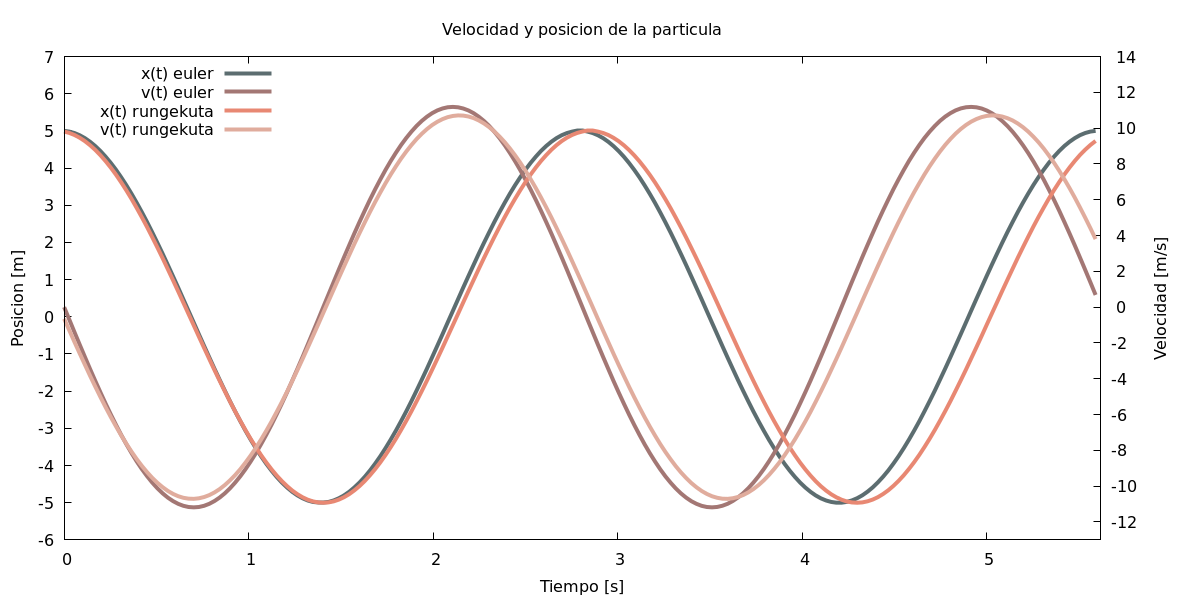
\includegraphics[scale=0.35]{images/velocidad-posicion.png}
        \caption{Gráfica de trayectorias para una partícula con las condiciones iniciales dadas.}
        \label{img}
    \end{figure}
    
    \begin{figure}[H]
        \centering
        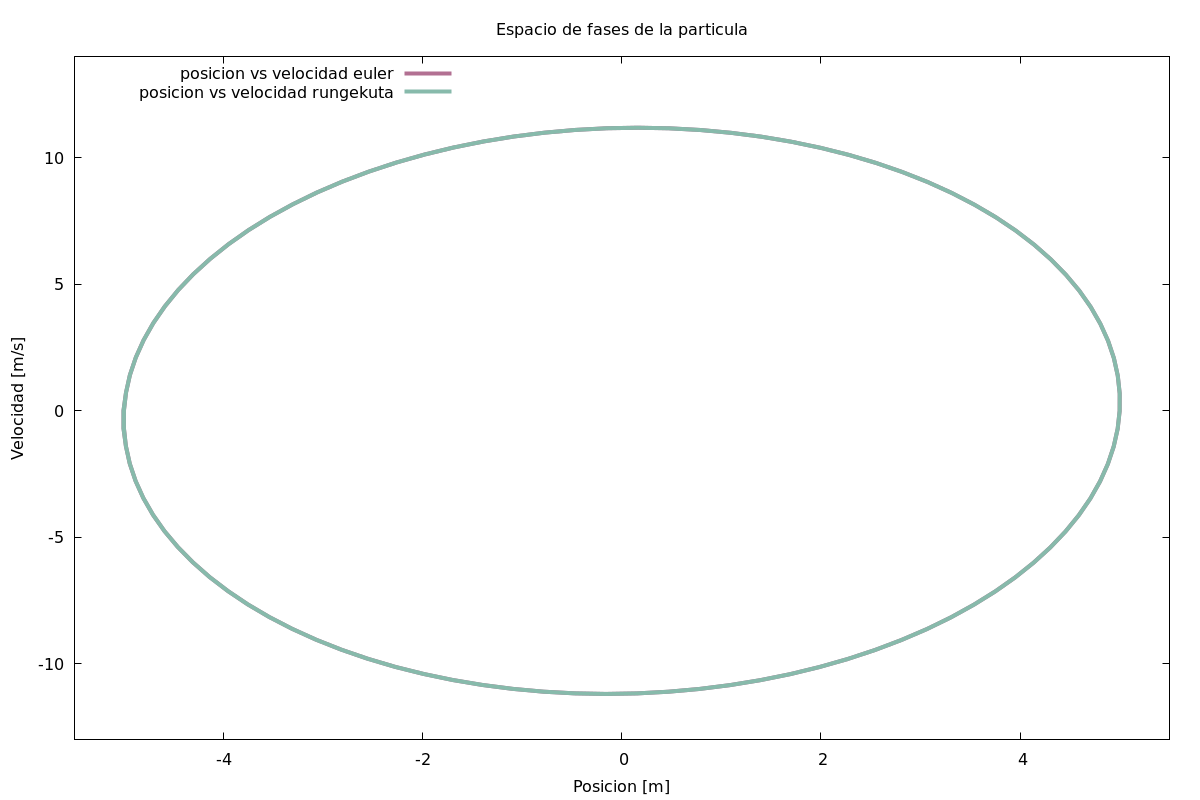
\includegraphics[scale=0.35]{images/espacio-fases.png}
        \caption{Gráfica de espacio de fases para partícula con condiciones iniciales dadas.}
        \label{img}
    \end{figure}
    
    
    \section{Animación del sistema masa-resorte.}
    
    Para realizar la animación se partió de utilizar los puntos ya calculados en la sección anterior, para esto se aprovechó la capacidad de \texttt{gnuplot} para graficar únicamente una fila en específico.
    
    La generación de cada uno de los fotogramas se llevó a cabo con la ayuda del siguiente método:
    
    \begin{verbatim}
string get_plt_content(int i)
{
    string name, content, range, number;

    size_t n = 3;
    number = to_string(i);
    number.insert(0, n - min(n, number.size()), '0');
    name = "./imgs/sequence/" + number + ".png";
    range = "every ::" + to_string(i) + "::" + to_string(i);

    if (i == 1)
        content = "set terminal pngcairo enhanced color size 1200,600\n";
    else
        content = "set terminal pngcairo transparent color size 1200,600\n";

    content += "set title \"Evolución de la posición\"\n";
    content += "set output '" + name + "'\n";
    content += "set xrange[0 : " + to_string(2 * T) + "]\n";
    content += "set yrange[-6:7]\n";
    content += "plot \"data.dat\" " + range + " i 0 u 1:2 w lp ps 1 pt 6 lc 8 t \"Posición Euler\"\n";
    content += "unset output\n";

    return content;
}
    \end{verbatim}
    
    este recibe un identificador que será dado por un contador que recorre desde cero hasta el número máximo de datos y retorna una cadena de texto que contiene el código \texttt{gnuplot} que permite realizar el fotograma $i$. Esta cadena de texto se guarda en un archivo \texttt{.plt} para ser ejecutado y posteriormente convertir las imágenes \texttt{.png} generadas a un único archivo \texttt{.gif}.\\

    \begin{verbatim}
void segundo_punto()
{
    ofstream outplt;
    outplt.open("./create-img/img-gif.plt");

    for (int i = 1; i <= n; i++)
    {
        outplt << get_plt_content(i);
    }

    system("gnuplot ./img-gif.plt");
    system("convert -delay 10 -loop 0 ./imgs/sequence/*.png ./imgs/trayectoria-gif.gif");
}
    \end{verbatim}    

    
    El resultado se puede ver en el siguiente enlace: \url{https://drive.google.com/drive/folders/10Btyv3v6Lqe-_LLd5ZaLdBRYMuEZHe7Z?usp=share_link}
    
    \begin{figure}[H]
        \centering
        \includegraphics[scale=0.35]{images/gif-resume.png}
        \caption{Vista previa y estática de la animación generada.}
        \label{img}
    \end{figure}
    
    
    
    
    \section{Pregunta.}
    
    Si lo que se desea es no únicamente cambiar el nombre de la imagen que se va a generar, sino que también crear un archivo \texttt{.plt} especifico para cada una, lo que se requiere es modificar también el nombre de archivo que se le pasa al \texttt{ofstream} creado.
    
    Este cambio se puede realizar modificando el \texttt{string} que se le pasa como parámetro al método \texttt{open} con lo cual se reutiliza el ciclo \texttt{for} que se planteó anteriormente, pero en vez de cambiar únicamente el nombre de la imagen, también cambiar el nombre del archivo. 
    
    \begin{verbatim}
void segundo_punto()
{
    ofstream outplt;

    for (int i = 1; i <= n; i++)
    {
        string fileName;
        fileName = "./create-img/img-gif" + to_string(i) + ".plt":
        outplt.open(fileName);
        
        outplt << get_plt_content(i);
        
        outplt.close():
    }

    ...
}
    \end{verbatim}
    
    Hay que tener en cuenta que para cambiar el nombre que es de tipo \texttt{string} se utiliza el identificador que es de tipo \texttt{int} por lo que es necesario convertir el identificador a texto, lo cual exige usar la función \texttt{to\_string} pero antes realizar el \texttt{\#include <string>}.
    
    
\end{document}